\chapter{IMPLÉMENTATION, RÉSULTATS ET DISCUSSION}
\begin{spacing}{1.2}
\minitoc
\thispagestyle{MyStyle}
\end{spacing}
\newpage

Dans ce chapitre, nous plongeons dans l'aspect pratique de notre projet, passant de la théorie à la mise en œuvre concrète. Nous commencerons par présenter l'environnement de développement utilisé, en mettant en lumière les outils, les bibliothèques et les configurations nécessaires à l'implémentation de notre modèle de prédiction. Ensuite, nous détaillerons l'architecture de l'application de prédiction, suivie du développement de l'application Web pour une utilisation conviviale. Enfin, nous examinerons les résultats obtenus et engagerons une discussion sur ces résultats, explorant également les perspectives futures de notre projet.

\section{Environnement de développement}

\subsection{Outils de développement}
Pour la réalisation de notre projet, nous avons opté pour un ensemble d'outils de développement qui ont été sélectionnés avec soin pour leur efficacité, leur polyvalence et leur adaptabilité aux exigences de notre tâche. Nous avons principalement utilisé le langage Python, l'environnement de développement VS Code, et Jupyter Notebook. Chacun de ces outils a été choisi pour des raisons spécifiques qui seront détaillées ci-dessous :

\subsubsection{Le langage python}
Python a été choisi comme langage de programmation principal pour plusieurs raisons. Tout d'abord, c'est un langage interprété, qui n'a pas besoin d'être compilé pour être exécuté, contrairement à des langages comme le C ou le C++, et de haut niveau. Il demande relativement peu de connaissances sur le fonctionnement d'un ordinateur pour être utilisé. Ensuite, Python est multiplateforme, c'est-à-dire qu'il fonctionne sur de nombreux systèmes d'exploitation : Windows, Mac OS X, Linux, Android, iOS, depuis les mini-ordinateurs Raspberry Pi jusqu'aux supercalculateurs. De plus, Python bénéficie d'une vaste bibliothèque de modules spécialisés pour le machine learning et le traitement de données par rapport à d'autres langages (Java, C++), tels que TensorFlow, Scikit-learn, PyTorch et Pandas, ce qui facilite grandement le développement de modèles d'intelligence artificielle. En outre, la communauté Python active et engagée offre un support continu ainsi qu'un accès à une multitude de ressources et de tutoriels, ce qui a été un atout précieux tout au long de notre projet.

\subsubsection{Visual Studio Code (VS Code)}
VS Code s'est imposé comme un environnement de développement de premier choix en raison de sa légèreté, de sa rapidité et de sa richesse en fonctionnalités. Son interface utilisateur intuitive et personnalisable offre une expérience de développement fluide, tout en offrant un large éventail d'extensions pour répondre à divers besoins de développement. De plus, VS Code prend en charge plusieurs langages de programmation, ce qui en fait un choix polyvalent pour travailler sur des projets multidisciplinaires. Enfin, la prise en charge native de Git et d'autres outils de contrôle de version a facilité la collaboration et la gestion du code source tout au long du cycle de développement.

\subsubsection{Jupyter Notebook}
Jupyter Notebook est une application Web open source qui permet de créer et de partager des documents comprenant du code en direct, des équations et d'autres ressources multimédias, utilisés dans plus de 40 langages de programmation, dont Python, Julia, Ruby, R, ou encore Scala. Nous l'avons utilisé dans notre projet pour l'analyse exploratoire des données ainsi que la modélisation statistique. Facile à utiliser, il permet d'exécuter le code cellule par cellule pour mieux comprendre son fonctionnement.

\subsection{Bibliothèques et librairie utilisées}
Dans le cadre de notre projet visant à prédire la réussite en licence des étudiants orientés en SEG à l'aide de l'intelligence artificielle, nous avons utilisé plusieurs bibliothèques Python spécialisées. Ces bibliothèques sont des outils essentiels pour la manipulation, l'analyse, la visualisation des données et la mise en œuvre des modèles d'apprentissage automatique. 

\subsubsection{NumPy}
NumPy est une bibliothèque fondamentale pour le calcul numérique en Python. Elle fournit des structures de données de tableau multidimensionnel (arrays) efficaces et performantes, ainsi que des fonctions mathématiques pour effectuer des opérations sur ces tableaux. Dans notre projet, NumPy est utilisé en combinaison avec Pandas pour effectuer des opérations de manipulation et de transformation de données plus rapides et efficaces. Les tableaux NumPy sont utilisés pour stocker et traiter les données avant de les convertir en DataFrames Pandas. De plus, NumPy est souvent utilisé en conjonction avec d'autres bibliothèques telles que Matplotlib et Scikit-learn pour effectuer des opérations mathématiques et des calculs numériques nécessaires à l'analyse des données et à la modélisation. En résumé, NumPy est une bibliothèque essentielle qui améliore les performances et la productivité lors de la manipulation et de l'analyse des données dans notre projet.

\subsubsection{Pandas}
Pandas est une bibliothèque open-source largement utilisée pour la manipulation et l'analyse des données en Python. Son principal objet est le DataFrame, une structure de données tabulaire puissante et flexible. Dans notre projet, Pandas est essentiel pour charger, nettoyer et prétraiter les données. Nous utilisons Pandas pour importer les jeux de données, traiter les valeurs manquantes, supprimer les doublons, filtrer les données et réaliser des opérations de fusion et de regroupement. Grâce à ses fonctionnalités avancées, Pandas simplifie la manipulation des données, ce qui permet un workflow plus fluide lors de la préparation des données pour l'analyse et la modélisation.

\subsubsection{Matplotlib}
Matplotlib est une bibliothèque de visualisation de données en Python qui permet de créer une grande variété de graphiques statiques, notamment des graphiques linéaires, des diagrammes à barres, des diagrammes circulaires, des histogrammes, etc. Dans notre projet, Matplotlib est utilisé pour visualiser les données d'entraînement et de test, ainsi que les résultats de la modélisation. Nous pouvons créer des graphiques pour explorer la distribution des variables, analyser les relations entre les caractéristiques et la variable cible, et évaluer les performances du modèle. Matplotlib offre une flexibilité et une personnalisation étendue, ce qui nous permet de créer des visualisations informatives et esthétiques pour communiquer nos résultats de manière efficace.

\subsubsection{Seaborn}
Seaborn est une bibliothèque de visualisation de données basée sur Matplotlib qui offre une interface plus conviviale et des styles de tracé esthétiques par défaut. Elle permet de créer rapidement des graphiques complexes et informatifs, notamment des diagrammes en violon, des tracés de régression linéaire et des matrices de corrélation. Dans notre projet, Seaborn complète Matplotlib en offrant des fonctionnalités supplémentaires pour explorer et visualiser les relations entre les variables. Nous utilisons Seaborn pour créer des graphiques qui mettent en évidence les tendances, les modèles et les corrélations dans nos données, ce qui nous aide à mieux comprendre le comportement des variables et à prendre des décisions plus éclairées lors de la modélisation.

\subsubsection{Scikit-learn}
Scikit-learn est une bibliothèque d'apprentissage automatique open-source qui offre une large gamme d'algorithmes d'apprentissage supervisé et non supervisé, ainsi que des outils pour l'évaluation et la validation des modèles. Dans notre projet, nous utilisons Scikit-learn pour construire, entraîner et évaluer notre modèle de prédiction. Nous avons choisi Scikit-learn pour sa simplicité d'utilisation, sa cohérence d'interface et sa grande efficacité. De plus, Scikit-learn propose une documentation exhaustive et une communauté active, ce qui en fait un choix populaire pour le développement d'applications d'apprentissage automatique en Python.

\subsubsection{Flask}
Flask est un framework web minimaliste pour Python qui permet de créer des applications Web légères et flexibles. Dans notre projet, nous utilisons Flask pour développer une interface utilisateur Web qui permettra aux utilisateurs de saisir les données et de générer des prédictions à partir du modèle entraîné. Flask offre des fonctionnalités pour gérer les requêtes HTTP, générer des pages Web dynamiques et interagir avec les modèles Python en arrière-plan. Nous avons choisi Flask pour sa simplicité, sa flexibilité et sa compatibilité avec les autres outils utilisés dans notre projet.

\subsection{Configuration des Outils et des Paramètres}
Pour garantir un développement efficace, nous avons configuré nos outils et nos paramètres selon les besoins spécifiques de notre projet. Cela comprend la configuration des environnements virtuels Python pour gérer les dépendances du projet, l'installation des extensions appropriées dans VS Code pour améliorer la productivité des développeurs, l'optimisation des paramètres de Jupyter Notebook pour assurer des performances optimales lors de l'exécution de code par cellules, et la configuration de Git comme système de contrôle de version pour notre projet qui nous a permis de gérer les différentes versions de notre code source et de suivre les modifications apportées aux fichiers.

\section{Présentation du modèle implémenté}
Après avoir développé une approche de solution dans le chapitre précédent, nous entrons maintenant dans la phase de concrétisation avec la présentation du modèle implémenté. Cette section se concentre sur la description détaillée de l'architecture de l'application de prédiction, la construction et les caractéristiques du modèle, ainsi que le développement de l'application web associée.

\subsection{Architecture du modèle implémenté}
L'architecture de notre modèle implémenté repose sur une approche modulaire et évolutive, conçue pour gérer efficacement les différentes étapes du processus de prédiction. Notre application est divisée en trois modules principaux : le module de prétraitement des données, le module de construction et d'entraînement du modèle, et le module de déploiement de l'application Web. 
\begin{itemize} 
	\item[\ding{118}] \textbf{Module de prétraitement des données} : il est chargé de nettoyer, normaliser et préparer les données brutes avant de les utiliser pour l'entraînement du modèle. Il comprend des fonctions pour détecter et traiter les valeurs aberrantes, gérer les données manquantes. 
	\item[\ding{118}] \textbf{Module de construction et d'entraînement du modèle} : ce module est responsable de la construction du modèle de prédiction à partir des données prétraitées. Il utilise des algorithmes d'apprentissage automatique cité dans le chapitre précédent. 
	\item[\ding{118}] \textbf{Module de déploiement de l'application web} : ce module prend en charge le déploiement de l'application web permettant aux utilisateurs de soumettre de nouvelles données et d'obtenir des prédictions en temps réel. 
\end{itemize}

\subsection{Implémentation du modèle}
 La mise en œuvre du modèle de prédiction repose sur les choix effectués lors de la phase de modélisation précédente. Nous utilisons les bibliothèques et les outils de développement mentionnés dans la section précédente pour entraîner le modèle sur les données prétraitées. Cette étape comprend la création d'un pipeline de prétraitement des données pour assurer la cohérence et la qualité des entrées du modèle. Nous explorons également les paramètres du modèle et les techniques d'optimisation pour améliorer ses performances prédictives.

\subsection{Développement de l’application Web} Le développement de notre application Web s'est appuyé sur le framework Flask pour sa simplicité, sa flexibilité et sa puissance. Nous avons utilisé Flask pour créer une API RESTful qui gère les requêtes des utilisateurs et communique avec notre modèle de prédiction. En plus de Flask, nous avons également utilisé HTML, CSS et Bootstrap pour concevoir et styliser l'interface utilisateur de l'application Web. Ainsi, l'application Web permet aux utilisateurs de soumettre des données sur les étudiants et d'obtenir des prédictions sur leur statut de réussite en temps réel. L'interface utilisateur est conviviale et intuitive, offrant une expérience utilisateur fluide et agréable.

\section{Résultats et discussions}

\subsection{Métrique et évaluation des modèles entraînés}
Pour évaluer l'efficacité de notre modèle de prédiction, nous avons utilisé plusieurs métriques de performance couramment utilisées dans le domaine de l'apprentissage automatique. Parmi ces métriques, nous avons notamment examiné la précision, le rappel, la F1-score et la matrice de confusion. Ces mesures nous ont permis d'évaluer la capacité du modèle à prédire avec précision la réussite en licence des étudiants orientés en économie. Les résultats obtenus sont présentés en détail dans les lignes qui suivent.

\subsubsection{Métrique de la performance}
\subsubsection*{Précision} La précision est une mesure qui évalue la proportion d'observations positives correctement prédites par le modèle parmi toutes les observations prédites comme positives. En d'autres termes, elle indique la capacité du modèle à éviter les faux positifs. Dans notre projet, la précision est cruciale, car elle nous permet de déterminer avec quelle fiabilité le modèle identifie correctement les étudiants qui réussissent effectivement leur licence. La formule de la précision est définie comme suit : \[ \text{Précision} = \frac{\text{Vrai\ Positif}}{\text{Vrai\ Positif} + \text{Faux\ Positif}} \]

\subsubsection*{Rappel} Le rappel, également appelé sensibilité ou recall en anglais, mesure la proportion d'observations positives correctement identifiées par le modèle parmi toutes les observations positives réelles. Il est important dans notre projet, car il nous indique la capacité du modèle à détecter les véritables positifs, c'est-à-dire les étudiants qui réussissent effectivement leur licence. La formule du rappel est la suivante : \[ \text{Rappel} = \frac{\text{Vrai\ Positif}}{\text{Vrai\ Positif} + \text{Faux\ Négatif}} \]

\subsubsection*{F1-Score}
Le F1-Score est une mesure qui combine à la fois la précision et le rappel en une seule valeur, offrant ainsi un équilibre entre les deux. Il est particulièrement utile lorsque les classes sont déséquilibrées, comme c'est souvent le cas dans les problèmes de classification binaire. Dans notre projet, le F1-Score nous permet d'évaluer globalement la performance du modèle en termes de précision et de rappel. La formule du F1-Score est définie comme suit :
\[ F1 = 2 \times \frac{\text{Précision} \times \text{Rappel}}{\text{Précision} + \text{Rappel}} \]

\subsubsection*{Matrice de confusion}
La matrice de confusion est une représentation tabulaire des prédictions du modèle par rapport aux valeurs réelles de la variable cible. Elle permet de visualiser les performances du modèle en termes de vrais positifs, vrais négatifs, faux positifs et faux négatifs. Cette métrique est essentielle dans notre projet, car elle fournit une vue détaillée des performances du modèle pour chaque classe de prédiction. La matrice de confusion n'a pas de formule spécifique, mais elle est générée à partir des prédictions du modèle et des valeurs réelles.

La matrice de confusion est une métrique essentielle qui permet d'évaluer les performances d'un modèle de prédiction en termes de vrais positifs, faux positifs, vrais négatifs et faux négatifs. Ces différentes classifications sont définies comme suit :

\begin{itemize}
	 \item[\ding{118}] \textbf{Vrai Positif (VP)} : cela correspond aux cas où le modèle prédit correctement qu'un étudiant a réussi sa licence et que cet étudiant a effectivement réussi.
	\item[\ding{118}] \textbf{Faux Positif (FP)} : dans ce cas, le modèle prédit à tort qu'un étudiant a réussi sa licence, alors qu'en réalité, cet étudiant a échoué.
	\item[\ding{118}] \textbf{Vrai Négatif (VN)} : ce sont les cas où le modèle prédit correctement qu'un 	étudiant a échoué à sa licence et que cet étudiant a effectivement échoué.
	\item[\ding{118}] \textbf{Faux Négatif (FN)} : Il s'agit des cas où le modèle prédit à tort qu'un étudiant a échoué à sa licence alors qu'en réalité, cet a effectivement réussi.
\end{itemize}

\begin{table}[H]%
    \center%
    \setlength{\fboxsep}{5pt}%
    \setlength{\fboxrule}{0.5pt}%
    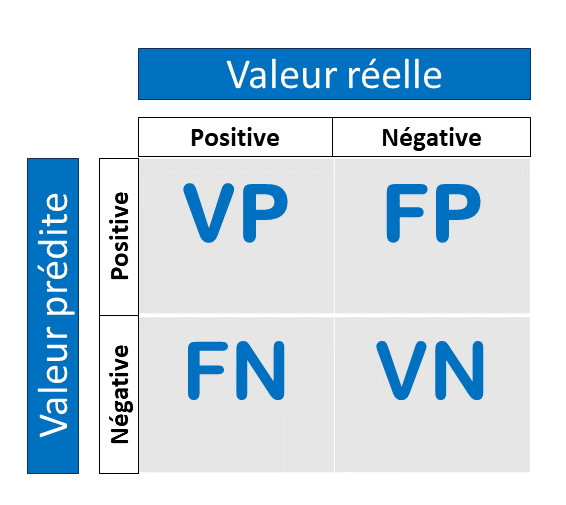
\includegraphics[width=9cm,height=6cm]{images/matrice de confusion.png}%
    \caption{Matrice de confusion.}%
\end{table}

\subsubsection{Évaluation des algorithmes entraînés}
Nous avons évalué les performances de nos différents algorithmes à l'aide des métriques d'évaluation précédemment définies afin de sélectionner celui offrant les meilleures prédictions. Cette évaluation s'est accompagnée de la génération de courbes et de graphiques pour une visualisation complète et comparative des performances des algorithmes.

\subsubsection*{Random Forest ou Forêt aléatoire}
\begin{minipage}[t]{0.5\textwidth}
    \begin{table}[H]
        \centering
        \setlength{\fboxsep}{5pt}
        \setlength{\fboxrule}{0.5pt}
        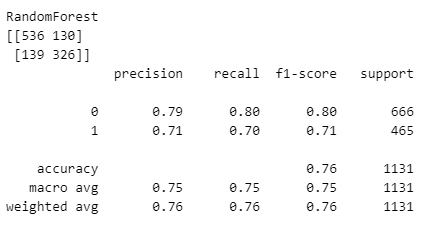
\includegraphics[width=7cm,height=5.4cm]{images/RandomForest.png}
        \caption{Matrice de confusion de Random Forest.}
    \end{table}
\end{minipage}
\begin{minipage}[t]{0.5\textwidth}
    \begin{figure}[H]
        \centering
        \setlength{\fboxsep}{5pt}
        \setlength{\fboxrule}{0.5pt}
        \fbox{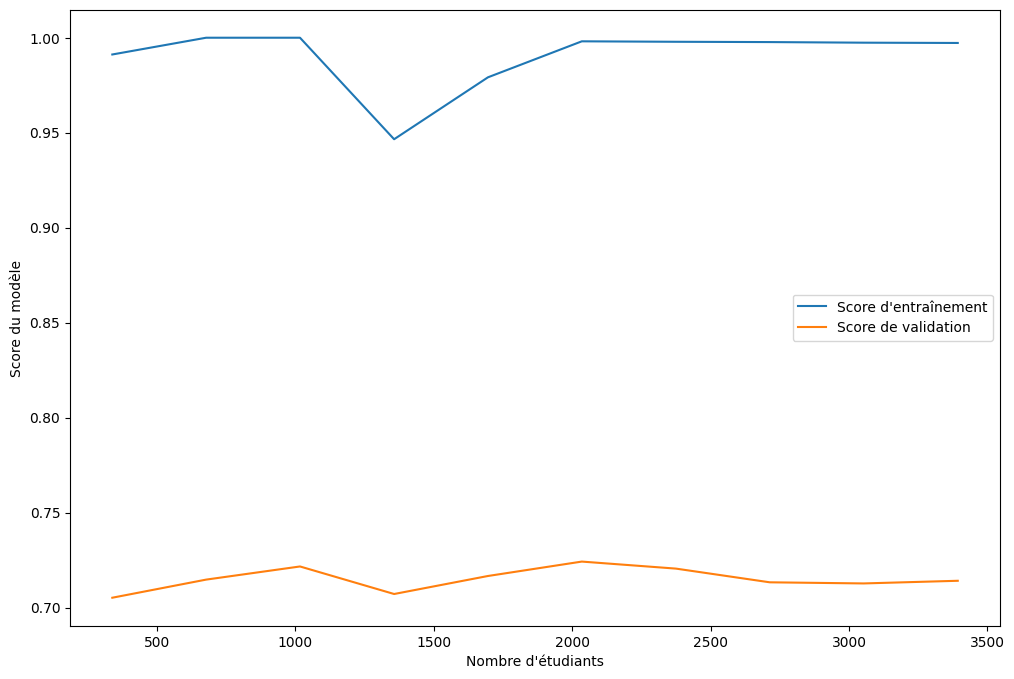
\includegraphics[width=7cm,height=5cm]{images/Evaluation RandomForest.png}}
        \caption{Courbe d'évaluation de Random Forest.}
    \end{figure}
\end{minipage}

\subsubsection*{Adaboost}
\begin{minipage}[t]{0.5\textwidth}
    \begin{table}[H]
        \centering
        \setlength{\fboxsep}{5pt}
        \setlength{\fboxrule}{0.5pt}
        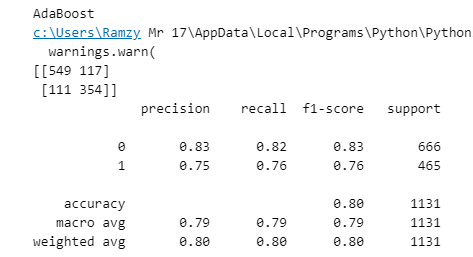
\includegraphics[width=7cm,height=5.36cm]{images/Adaboost.png}
        \caption{Matrice de confusion de Adaboost.}
    \end{table}
\end{minipage}
\begin{minipage}[t]{0.5\textwidth}
    \begin{figure}[H]
        \centering
        \setlength{\fboxsep}{5pt}
        \setlength{\fboxrule}{0.5pt}
        \fbox{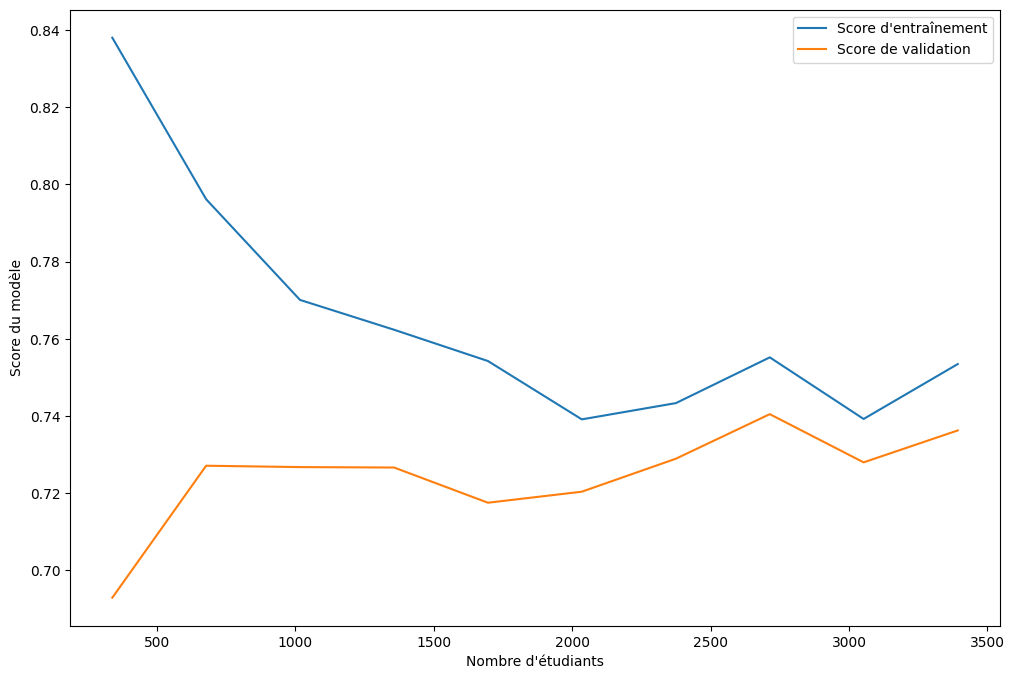
\includegraphics[width=7cm,height=5cm]{images/Evaluation Adaboost.png}}
        \caption{Courbe d'évaluation de Adaboost.}
    \end{figure}
\end{minipage}

\subsubsection*{SVM}
\begin{minipage}[t]{0.5\textwidth}
    \begin{table}[H]
        \centering
        \setlength{\fboxsep}{5pt}
        \setlength{\fboxrule}{0.5pt}
        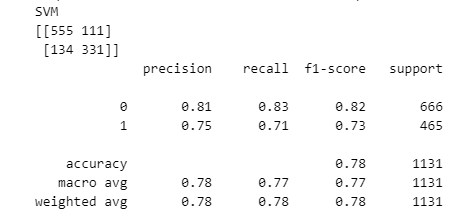
\includegraphics[width=7cm,height=5.36cm]{images/SVM.png}
        \caption{Matrice de confusion de SVM.}
    \end{table}
\end{minipage}
\begin{minipage}[t]{0.5\textwidth}
    \begin{figure}[H]
        \centering
        \setlength{\fboxsep}{5pt}
        \setlength{\fboxrule}{0.5pt}
        \fbox{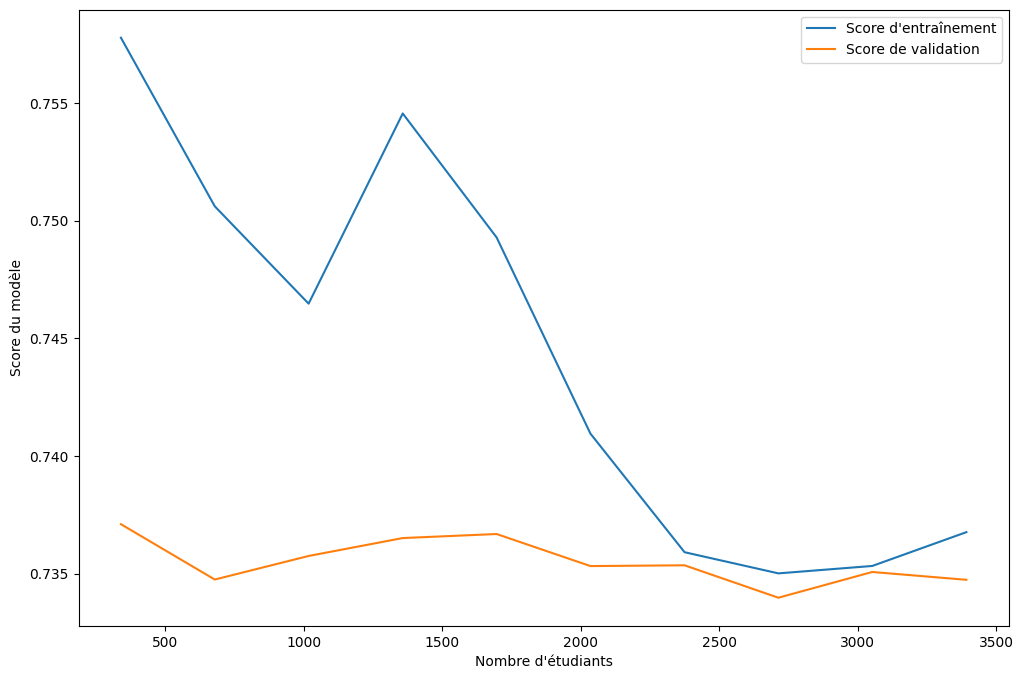
\includegraphics[width=7cm,height=5cm]{images/Evaluation SVM.png}}
        \caption{Courbe d'évaluation de SVM.}
    \end{figure}
\end{minipage}

\subsubsection*{KNN}
\begin{minipage}[t]{0.5\textwidth}
    \begin{table}[H]
        \centering
        \setlength{\fboxsep}{5pt}
        \setlength{\fboxrule}{0.5pt}
        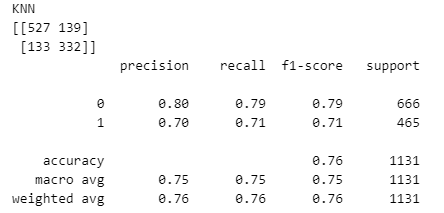
\includegraphics[width=7cm,height=5.37cm]{images/KNN (1).png}
        \caption{Matrice de confusion de KNN.}
    \end{table}
\end{minipage}
\begin{minipage}[t]{0.5\textwidth}
    \begin{figure}[H]
        \centering
        \setlength{\fboxsep}{5pt}
        \setlength{\fboxrule}{0.5pt}
        \fbox{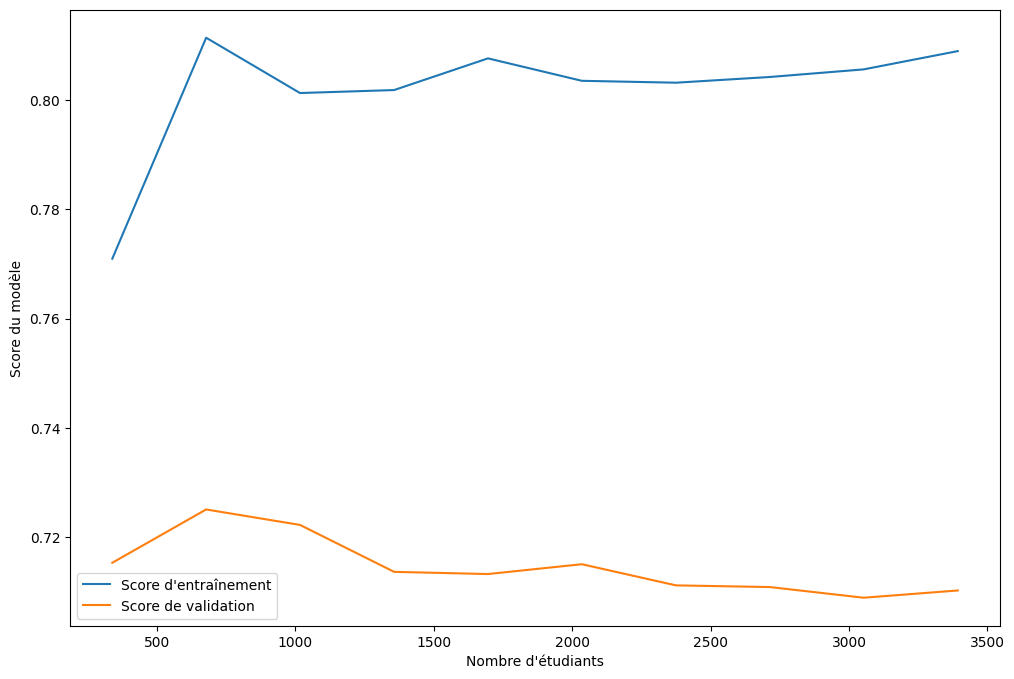
\includegraphics[width=7cm,height=5cm]{images/Evaluation KNN.png}}
        \caption{Courbe d'évaluation de KNN.}
    \end{figure}
\end{minipage}
\newpage
\subsubsection*{Arbre de décision}
\begin{minipage}[t]{0.5\textwidth}
    \begin{table}[H]
        \centering
        \setlength{\fboxsep}{5pt}
        \setlength{\fboxrule}{0.5pt}
        \includegraphics[width=7cm,height=5.37cm]{images/Abre de décision.png}
        \caption{Matrice de confusion de Arbre de décision.}
    \end{table}
\end{minipage}
\begin{minipage}[t]{0.5\textwidth}
    \begin{figure}[H]
        \centering
        \setlength{\fboxsep}{5pt}
        \setlength{\fboxrule}{0.5pt}
        \fbox{\includegraphics[width=7cm,height=5cm]{images/Evaluation Abre de décision.png}}
        \caption{Courbe d'évaluation de Arbre de décision.}
    \end{figure}
\end{minipage}

\subsubsection*{Réseaux de neurones}
\begin{minipage}[t]{0.5\textwidth}
    \begin{table}[H]
        \centering
        \setlength{\fboxsep}{5pt}
        \setlength{\fboxrule}{0.5pt}
        \includegraphics[width=7cm,height=5.37cm]{images/Réseau de neurones.png}
        \caption{Matrice de confusion de Réseaux de neurones.}
    \end{table}
\end{minipage}
\begin{minipage}[t]{0.5\textwidth}
    \begin{figure}[H]
        \centering
        \setlength{\fboxsep}{5pt}
        \setlength{\fboxrule}{0.5pt}
        \fbox{\includegraphics[width=7cm,height=5cm]{images/Evaluation Réseau de neurones.png}}
        \caption{Courbe d'évaluation de Réseaux de neurones.}
    \end{figure}
\end{minipage}
\newpage
Nous pouvons résumer les métriques d'évaluation des différents algorithmes dans le tableau ci-dessous :

\begin{table}[h]
\centering
\begin{tabular}{lccc}
\hline
Algorithme & Précision & Rappel & F1-score \\
\hline
\textit{Random Forest} & 75\% & 75\% & 75\% \\
\textit{Adaboost} & 79\% & 79\% & 79\% \\
\textit{SVM} & 78\% & 77\% & 77\% \\
\textit{KNN} & 75\% & 75\% & 75\% \\
\textit{Arbre de décision} & 71\% & 71\% & 71\% \\
\textit{Réseaux de neurones} & 80\% & 80\% & 80\% \\
\hline
\end{tabular}
\caption{Métriques d'évaluation des algorithmes.}

\end{table}

L'analyse du tableau des métriques d'évaluation des différents algorithmes permet de comparer les performances de chaque algorithme en termes de précision, rappel et F1-score. Ces observations suggèrent que les réseaux de neurones pourraient être l'algorithme le plus prometteur pour la tâche spécifique évaluée, en raison de leur performance globalement supérieure sur les trois métriques d'évaluation. Il est important de noter que ces résultats serviront de base pour l'optimisation future des hyperparamètres, permettant ainsi d'améliorer davantage les performances des algorithmes et ce que nous obtenons.

\begin{minipage}[t]{0.5\textwidth}
    \begin{table}[H]
        \centering
        \setlength{\fboxsep}{5pt}
        \setlength{\fboxrule}{0.5pt}
        \includegraphics[width=7cm,height=5.37cm]{images/Réseau de neurone opti.png}
        \caption{Matrice de confusion de Réseaux de neurones avec les hyperparamètres.}
    \end{table}
\end{minipage}
\begin{minipage}[t]{0.5\textwidth}
    \begin{figure}[H]
        \centering
        \setlength{\fboxsep}{5pt}
        \setlength{\fboxrule}{0.5pt}
        \fbox{\includegraphics[width=7cm,height=5cm]{images/Validation Réseau de neurone.png}}
        \caption{Courbe d'évaluation de Réseaux de neurones.}
    \end{figure}
\end{minipage}

\subsection{Déploiement du modèle}
Après avoir opté pour le modèle des Réseaux de neurones, nous l'avons déployé en utilisant la technologie Web. L'objectif de cette démarche était de développer une interface graphique permettant de visualiser les résultats des tests du modèle retenu. Cela visait à offrir aux nouveaux étudiants de l'UNZ, souhaitant évaluer leurs chances de réussite en licence économie, la possibilité de prédire leur succès. Ainsi, nous avons élaboré une interface Web basée sur Flask. La capture d'écran ci-dessous présente la page d'accueil, permettant aux utilisateurs d'exploiter le modèle pour prédire leurs chances de réussite.

\begin{figure}[H]%
    \center%
    \setlength{\fboxsep}{5pt}%
    \setlength{\fboxrule}{0.5pt}%
    \fbox{
    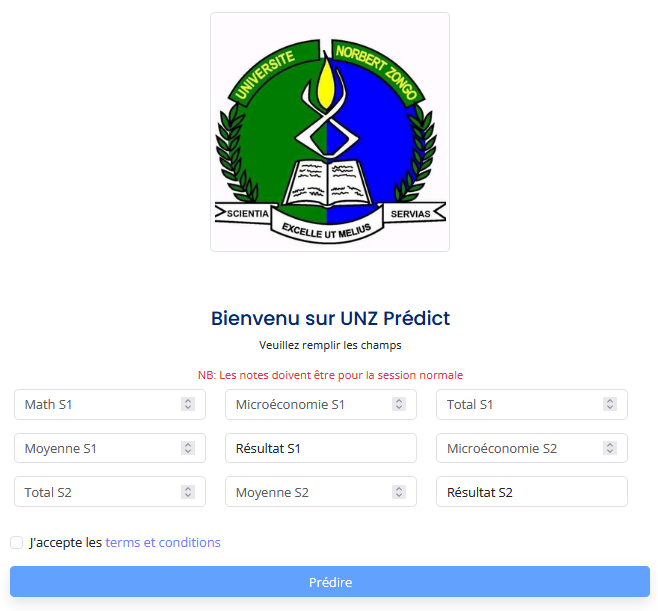
\includegraphics[width=10cm,height=11cm]{images/Unz predict.png}%
    }
    \caption{Page d’accueil de l’application Web.}%
\end{figure}
Une fois sur la page d'accueil présentée ci-dessus, l'utilisateur remplira le formulaire puis cliquera sur le bouton "Prédire". Il est à noter que les champs de ce formulaire sont des zones de saisie ou "input".

\subsection{Résultat de l'application}
Avant de mettre en production une application destinée à aider les étudiants à évaluer leurs chances de réussite en licence économie à l'UNZ, il est essentiel de la soumettre à des tests rigoureux pour garantir son bon fonctionnement et sa fiabilité. Dans cette section, nous décrirons en détail les différents tests auxquels l'application a été soumise, ainsi que les résultats obtenus. Ces tests ont été réalisés dans le but d'assurer que l'application réponde aux attentes des utilisateurs et fournisse des prédictions précises et pertinentes pour leur réussite académique.

\begin{figure}[H]%
    \center%
    \setlength{\fboxsep}{5pt}%
    \setlength{\fboxrule}{0.5pt}%
    \fbox{
    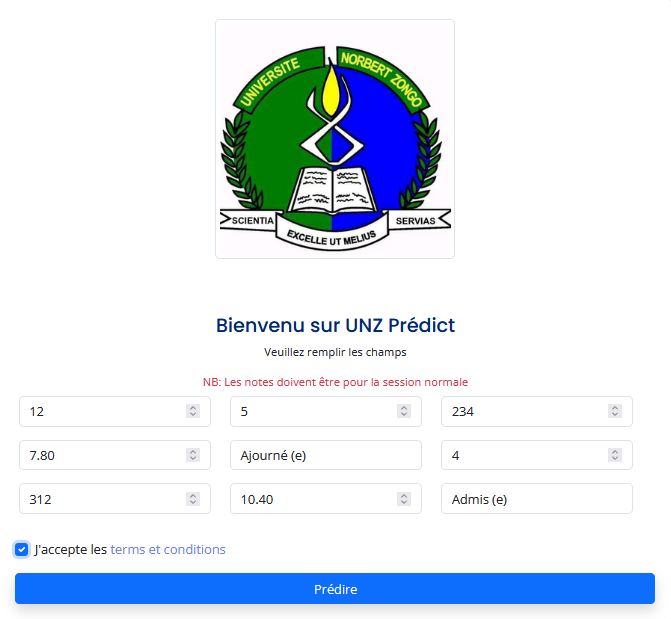
\includegraphics[width=8cm,height=9cm]{images/Forme1.png}%
    }
    \caption{Exemple de prédiction 1.}%
\end{figure}

\begin{figure}[H]%
    \center%
    \setlength{\fboxsep}{5pt}%
    \setlength{\fboxrule}{0.5pt}%
    \fbox{
    \includegraphics[width=8cm,height=9cm]{images/Résultat1.png}%
    }
    \caption{Résultat de la prédiction 1.}%
\end{figure}

Pour le cas de l'exemple de la figure 4.9, il s'agit d'un étudiant dont les résultats sont les suivants : 12 en mathématiques au semestre 1, 5 en microéconomie au semestre 1, avec un total de 234 points et une moyenne de 7,80 au semestre 1, résultant en un échec au semestre 1. Au semestre 2, l'étudiant obtient 4 en Microéconomie, un total de 312 points et une moyenne de 10,40, ce qui conduit à une réussite au semestre 2. Le modèle de prédiction estime que cet étudiant a 20,76\% de chance de réussir sa licence, ce qui veut dire qu'il va échouer.
\begin{figure}[H]%
    \center%
    \setlength{\fboxsep}{5pt}%
    \setlength{\fboxrule}{0.5pt}%
    \fbox{
    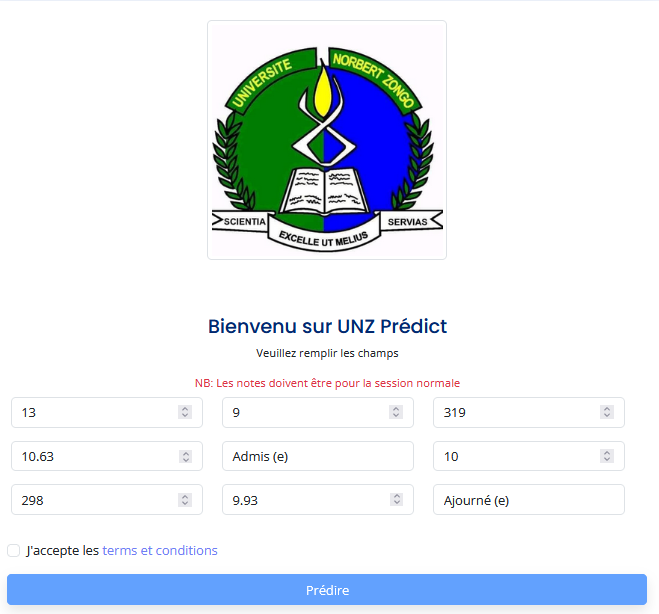
\includegraphics[width=8cm,height=9cm]{images/Forme2.png}%
    }
    \caption{Exemple de prédiction 2.}%
\end{figure}

\begin{figure}[H]%
    \center%
    \setlength{\fboxsep}{5pt}%
    \setlength{\fboxrule}{0.5pt}%
    \fbox{
    \includegraphics[width=8cm,height=9cm]{images/Résultat2.png}%
    }
    \caption{Résultat de la prédiction 2.}%
\end{figure}

Pour le cas de l'exemple de la figure 4.11, il s'agit d'un étudiant dont les résultats sont les suivants : 13 en mathématiques au semestre 1, 9 en microéconomie au semestre 1, avec un total de 319 points et une moyenne de 10.63 au semestre 1, résultant en une réussite au semestre 1. Au semestre 2, l'étudiant obtient 10 en microéconomie, un total de 298 points et une moyenne de 9.93, ce qui conduit à un échec au semestre 2. Le modèle de prédiction estime que cet étudiant a 69.14\% de chance de réussir sa licence, ce qui veut dire qu'il va réussir.

\subsection{Perspectives futures}
Enfin, en ce qui concerne les perspectives futures, nous envisageons plusieurs axes d'amélioration et d'extension de notre travail. Cela comprend l'exploration de techniques d'apprentissage automatique plus avancées, telles que les réseaux de neurones profonds, pour améliorer les performances prédictives du modèle. Nous prévoyons également d'enrichir les fonctionnalités de l'application Web en intégrant des analyses visuelles interactives et en développant des fonctionnalités de recommandation personnalisée. De plus, nous envisageons d'étendre notre étude à d'autres filières universitaires afin de généraliser notre approche à un plus large éventail de domaines.

\section{Conclusion}

Ce chapitre marque la concrétisation de notre projet, en passant de la conceptualisation à la mise en œuvre. Nous avons détaillé l'environnement de développement utilisé, l'architecture de notre application de prédiction, et présenté les résultats obtenus. En analysant ces résultats, nous avons également ouvert la porte à des perspectives futures, soulignant les opportunités d'amélioration et d'extension de notre travail. En somme, ce chapitre apporte une contribution tangible à notre projet, en le rendant opérationnel et en ouvrant la voie à de nouvelles avenues de recherche et de développement.
